\section{Experimental Results and Discussions}
\label{sec:results_discussion}

\subsection{Global Surrogate Model Performance}
\label{subsec:global_surrogate_results}

Tables~\ref{tab:global_feasibility_results} and~\ref{tab:global_steel_results} compare the three surrogate models under progressively enriched input settings. For feasibility prediction, the Param-MLP achieves a PR-AUC of 0.6137 and an F1 score of 0.5927 on unseen layouts. Incorporating global layout statistics substantially improves these values to 0.8163 and 0.7370, corresponding to relative improvements of 33.0\% and 24.3\%, respectively. This result indicates that layout-level geometric information is essential for cross-layout prediction. The proposed FuseGNN further increases the PR-AUC to 0.8593 and the F1 score to 0.7688, indicating that the room-level graph captures spatial and topological information that cannot be fully represented by manually defined global statistics.

More importantly, the FuseGNN provides a favorable balance between candidate rejection and feasible-solution retention. Under the selected screening threshold, it rejects approximately 47.36\% of the candidates while maintaining a feasibility recall of 0.9998, with only three feasible samples falsely rejected. This conservative screening performance is substantially better than that of the parameter-only model and also improves upon the statistics-based model, supporting its use for removing low-feasibility candidates before FEA.

A similar pattern is observed for reinforcement prediction. The Param-MLP produces an MAE of 32.30~t and an $R^2$ of 0.351, confirming that design parameters alone are insufficient to represent layout-dependent reinforcement demand. Adding global layout statistics reduces the MAE to 13.83~t, while the FuseGNN further lowers it to 11.48~t and increases the $R^2$ to 0.924. It also achieves high pairwise ranking accuracy, Spearman correlation, and top-10\% recall. Since the reinforcement surrogate is primarily used for candidate ranking rather than exact quantity estimation, these results demonstrate that the proposed representation can reliably identify candidates with relatively low reinforcement demand within each layout.

Fig.~\ref{fig:global_surrogate_overview} further illustrates the prediction behavior of the FuseGNN. The precision-recall curve in Fig.~\ref{fig:global_surrogate_overview}(a) shows that the graph-based feasibility model achieves a much better precision-recall trade-off than the baseline feasible rate. However, the layout-wise probability comparison in Fig.~\ref{fig:global_surrogate_overview}(b) reveals that prediction bias still exists for some layouts. Several layouts with low true feasible rates are assigned overly optimistic feasibility probabilities. The reinforcement error distribution in Fig.~\ref{fig:global_surrogate_overview}(d) also shows that the prediction error becomes more biased in high-reinforcement regions. In the highest 20\% reinforcement-usage interval, the MAE increases to approximately 20.7~t and the bias reaches about $-17.4$~t. Therefore, although the FuseGNN model provides effective feasibility screening and reinforcement ranking, its layout and demand dependent errors make it insufficient for direct optimization without further calibration.


\begin{table}[!t]
\centering
\setcounter{table}{4}
\caption{Representative local calibration results and local-only ablation using 100 FEA-verified samples.}
\label{tab:local_calibration_results}
\setlength{\tabcolsep}{2pt}
\begin{threeparttable}
\begin{tabularx}{\columnwidth}{@{}>{\raggedright\arraybackslash}X>{\centering\arraybackslash}p{0.14\columnwidth}>{\centering\arraybackslash}p{0.17\columnwidth}>{\centering\arraybackslash}p{0.16\columnwidth}>{\centering\arraybackslash}p{0.13\columnwidth}@{}}
\toprule
Metric & Global & Local only & Calib. & Improv. \\
\midrule
\multicolumn{5}{@{}l}{\textit{Feasibility}} \\
Brier & 0.0749 & 0.0755 & 0.0437 & 42\% \\
ECE & 0.0895 & 0.0451 & 0.0333 & 63\% \\
feasibility recall & 0.9990 & 0.7265 & 0.9939 & -1\% \\
reject rate & 0.4708 & 0.5639 & 0.5481 & 16\% \\
\midrule
\multicolumn{5}{@{}l}{\textit{Steel}} \\
MAE & 11.48~t & 4.82~t & 2.04~t & 82\% \\
RMSE & 12.30~t & 5.64~t & 2.76~t & 78\% \\
$R^2$ & 0.847 & 0.976 & 0.994 & 17\% \\
MAPE & 9.26\% & 3.26\% & 1.64\% & 82\% \\
\bottomrule
\end{tabularx}

\begin{tablenotes}[flushleft]
\footnotesize
\item \textit{Note:} Global: uncalibrated global surrogate; Local only: model trained directly on current-layout samples without global predictions; Calib.: proposed local calibration of the global surrogate; Improv.: relative change from Global to Calib.
\end{tablenotes}

\end{threeparttable}
\end{table}
% \setcounter{table}{6}


\begin{table*}[!t]
\centering
\setcounter{table}{5}
\caption{Optimization efficiency and solution quality under different candidate evaluation strategies.}
\label{tab:optimization_summary_results}
\small
\setlength{\tabcolsep}{3.5pt}
\begin{tabularx}{\textwidth}{@{}>{\raggedright\arraybackslash}p{0.13\textwidth}
>{\raggedright\arraybackslash}p{0.13\textwidth}
>{\centering\arraybackslash}p{0.055\textwidth}
>{\centering\arraybackslash}p{0.095\textwidth}
>{\centering\arraybackslash}X
>{\centering\arraybackslash}p{0.105\textwidth}
>{\centering\arraybackslash}X
>{\centering\arraybackslash}p{0.12\textwidth}@{}}
\toprule
Algorithm & Method & Runs & Success rate & Mean FEA calls & FEA reduction & First feasible FEA & Cost ratio vs. full \\
\midrule
\multirow{3}{*}{GA}
& Full FEA & 75 & 68.0\% & 650 & -- & 72 & -- \\
& Cost ranking & 75 & 60.0\% & 279 & 57.0\% & 24 & 1.016 \\
& Screen \& ranking & 75 & 65.3\% & 223 & 65.7\% & 28 & 1.018 \\
\midrule
\multirow{3}{*}{PSO}
& Full FEA & 75 & 61.3\% & 573 & -- & 105 & -- \\
& Cost ranking & 75 & 57.3\% & 261 & 54.4\% & 56 & 1.006 \\
& Screen \& ranking & 75 & 58.7\% & 215 & 62.4\% & 51 & 1.017 \\
\midrule
\multirow{3}{*}{Random search}
& Full FEA & 75 & 68.0\% & 717 & -- & 71 & -- \\
& Cost ranking & 75 & 66.7\% & 358 & 50.1\% & 42 & 1.000 \\
& Screen \& ranking & 75 & 66.7\% & 247 & 65.6\% & 31 & 1.002 \\
\bottomrule
\end{tabularx}

\vspace{0.8em}

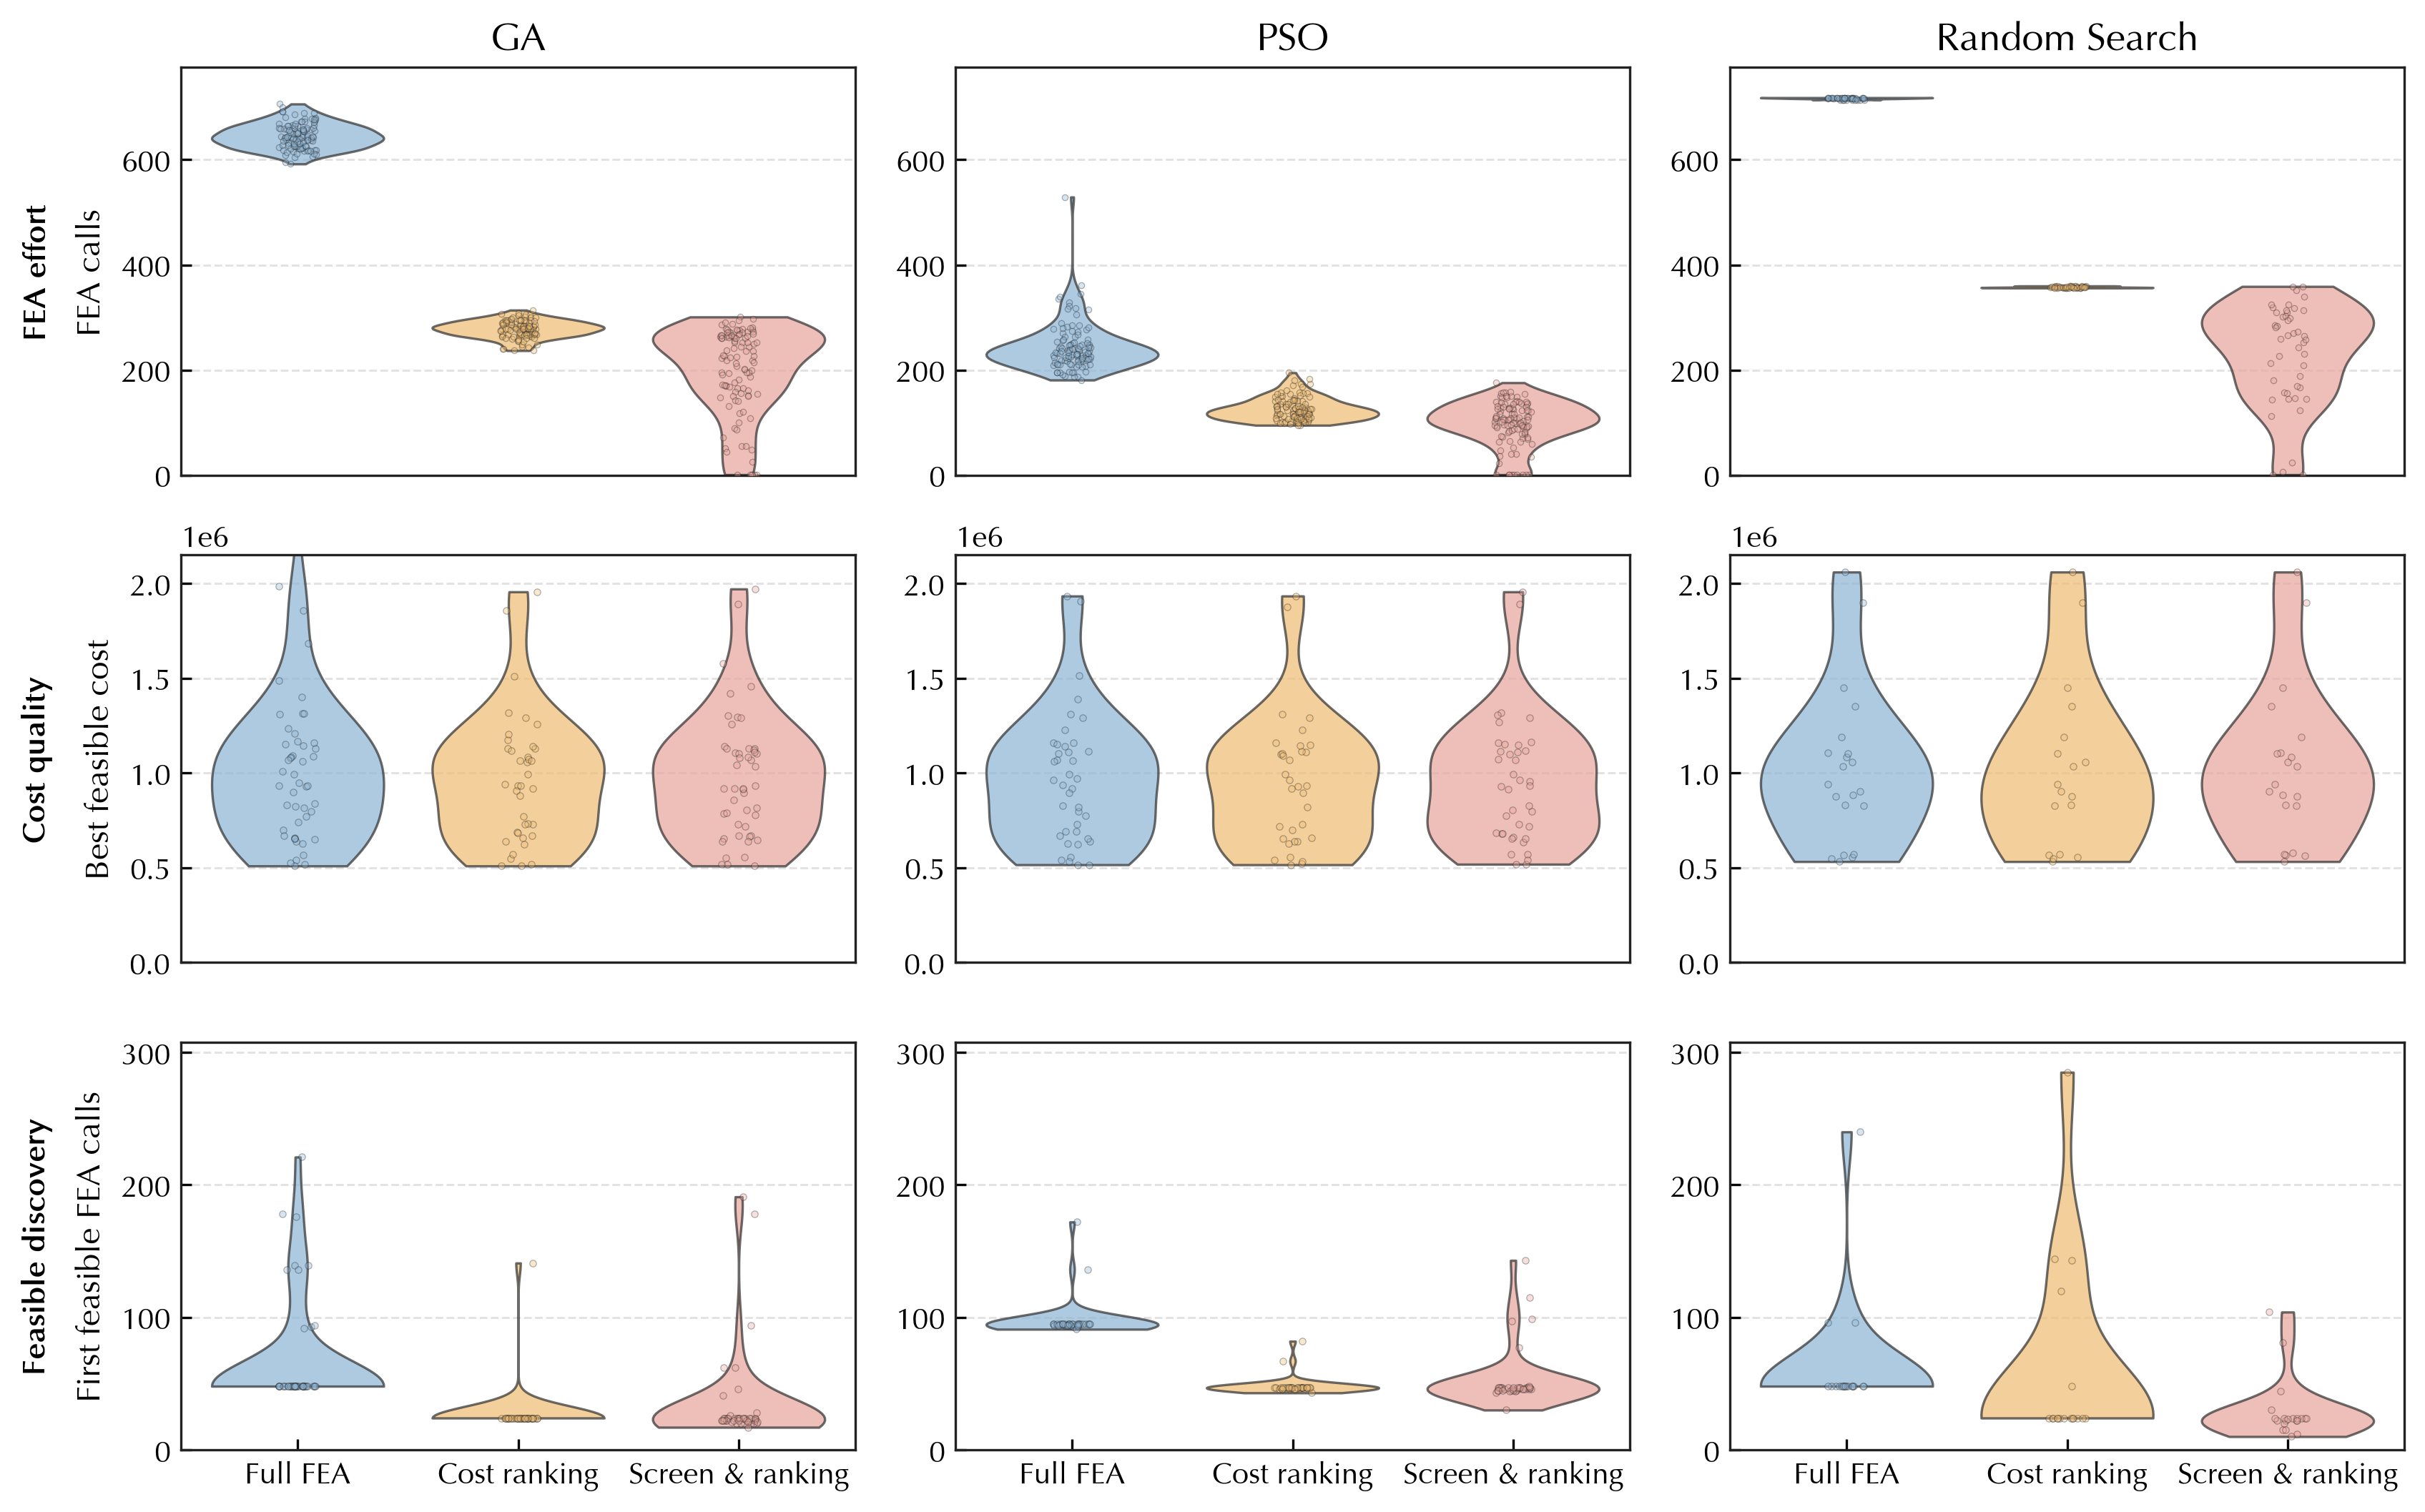
\includegraphics[width=\textwidth]{optimization_benchmark_results.pdf}
\captionsetup{labelfont=normalfont,textfont=normalfont,labelsep=colon,justification=centering,singlelinecheck=true}
\captionof{figure}{Optimization efficiency and solution quality under different optimizers and candidate evaluation strategies.}
\label{fig:optimization_benchmark_results}
\end{table*}

\begin{figure*}[t]
\centering
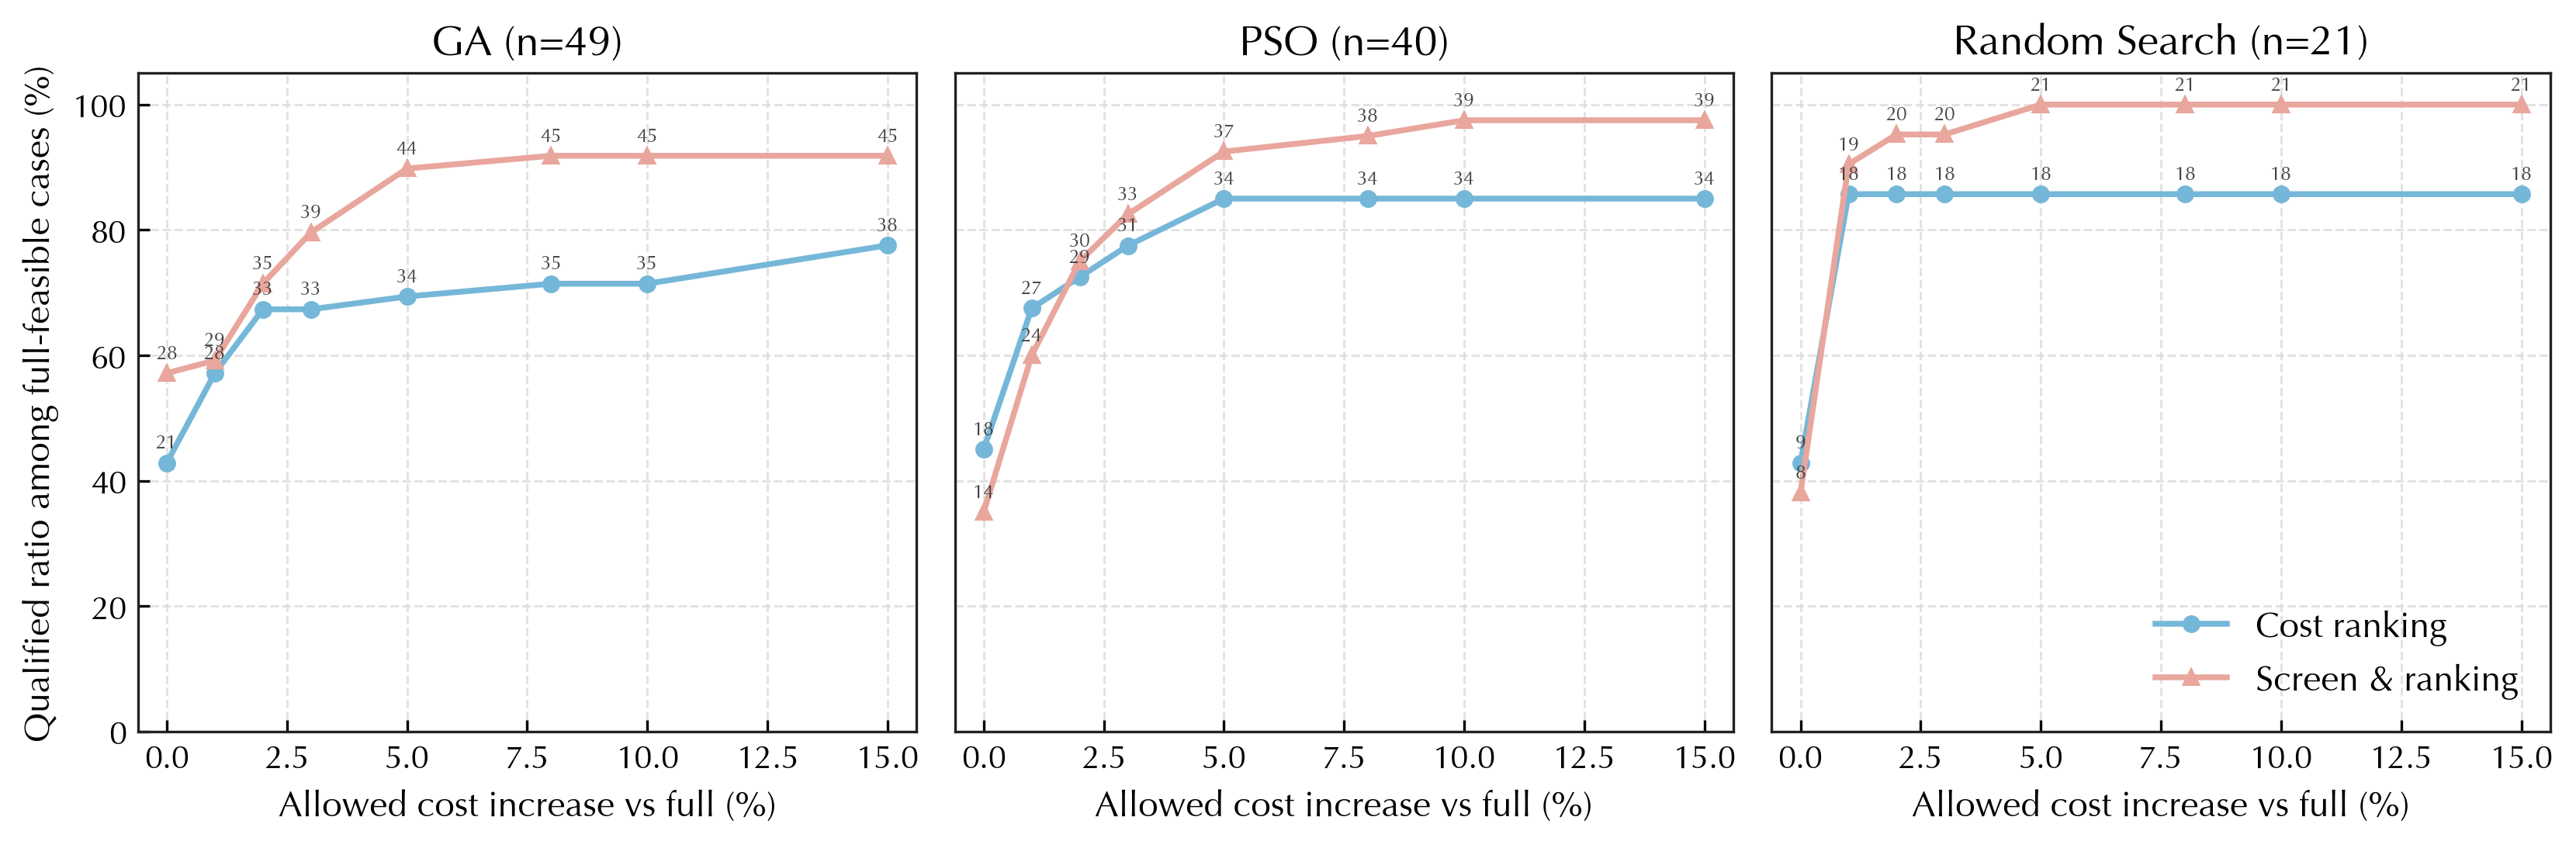
\includegraphics[width=\textwidth]{cost_tolerance_analysis.pdf}
\caption{Cost-tolerance analysis of surrogate-informed strategies in full-feasible cases.}
\label{fig:cost_tolerance_analysis}
\end{figure*}

\begin{figure*}[t]
\centering
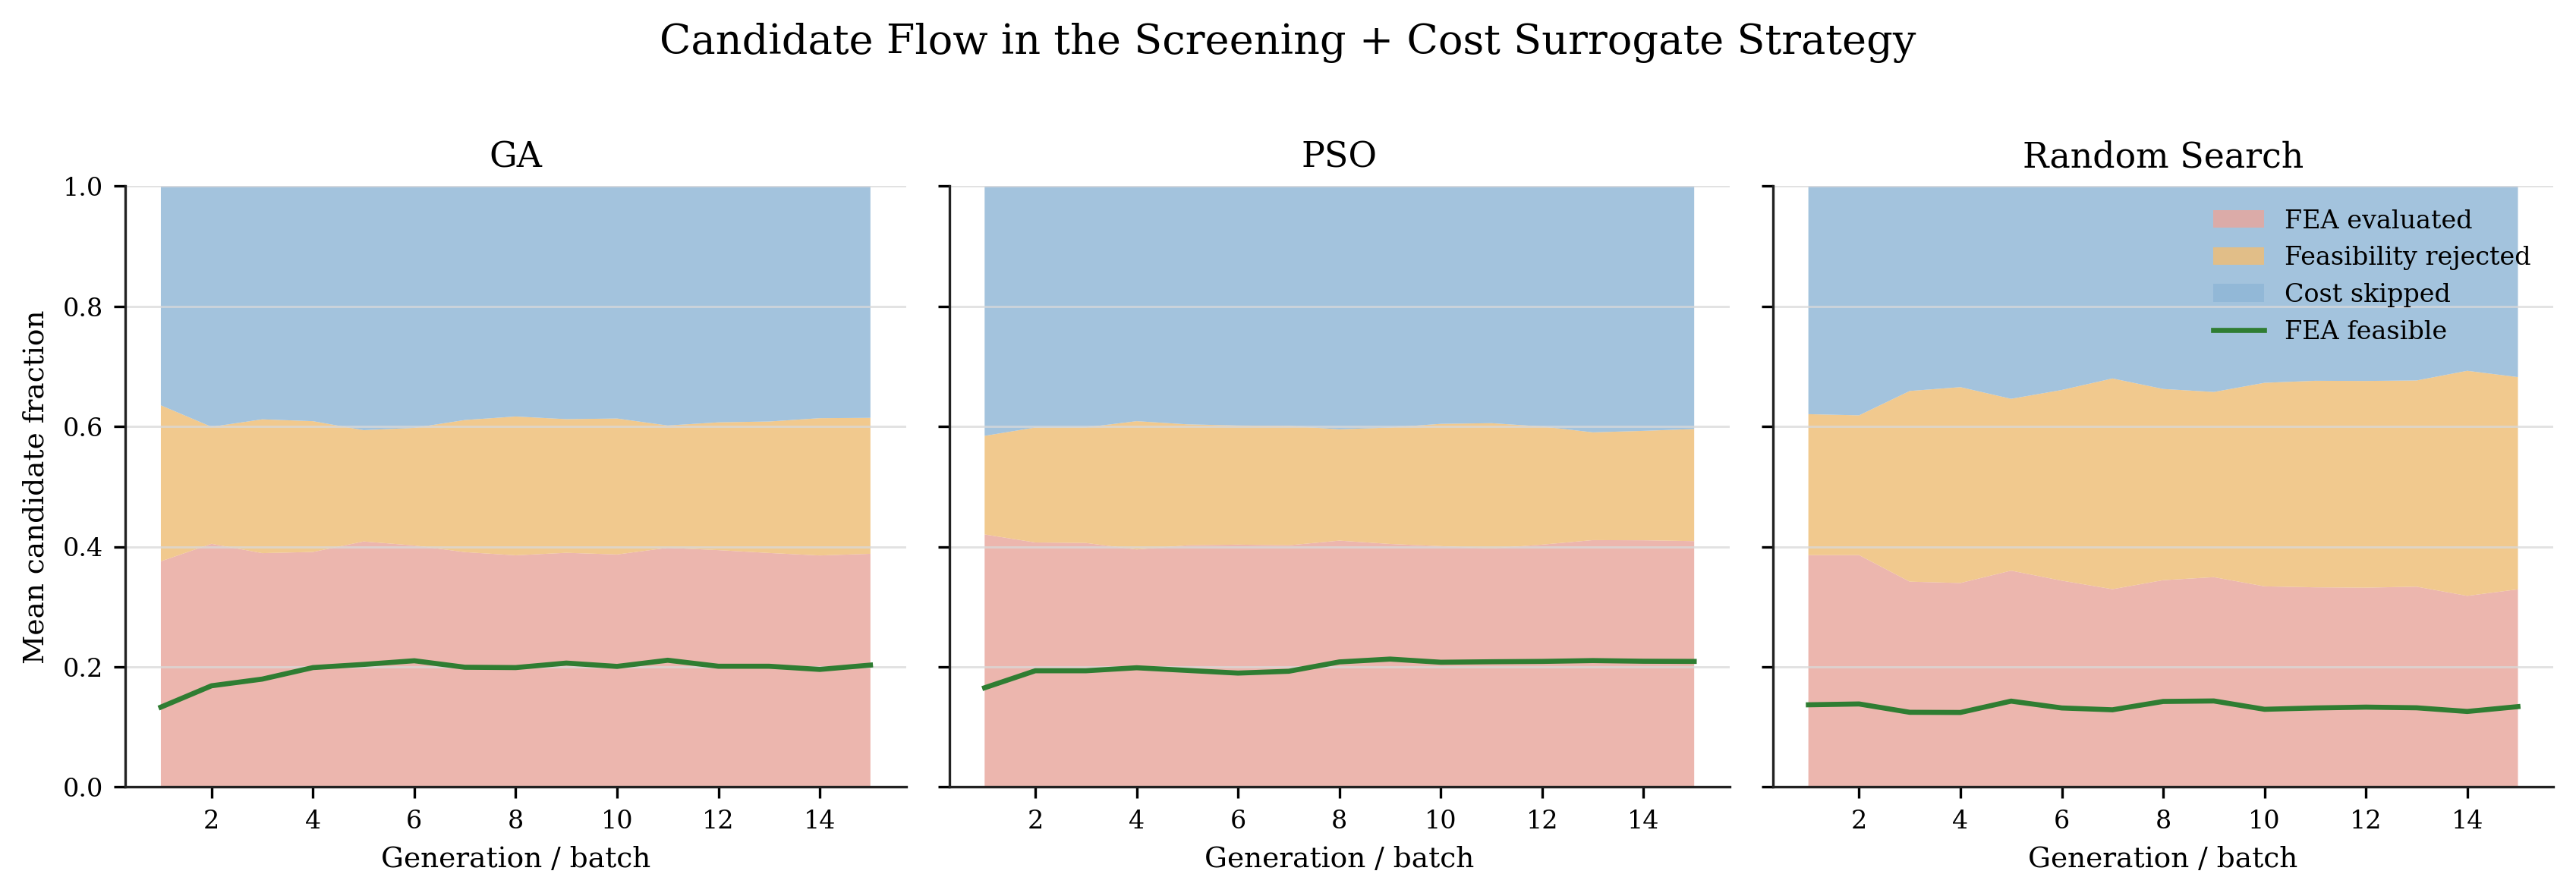
\includegraphics[width=\textwidth,height=0.25\textheight,keepaspectratio]{candidate_flow_analysis.pdf}
\caption{Candidate flow in the calibrated surrogate-informed optimization process.}
\label{fig:candidate_flow_analysis}
\end{figure*}

\begin{figure*}[!t]
\centering
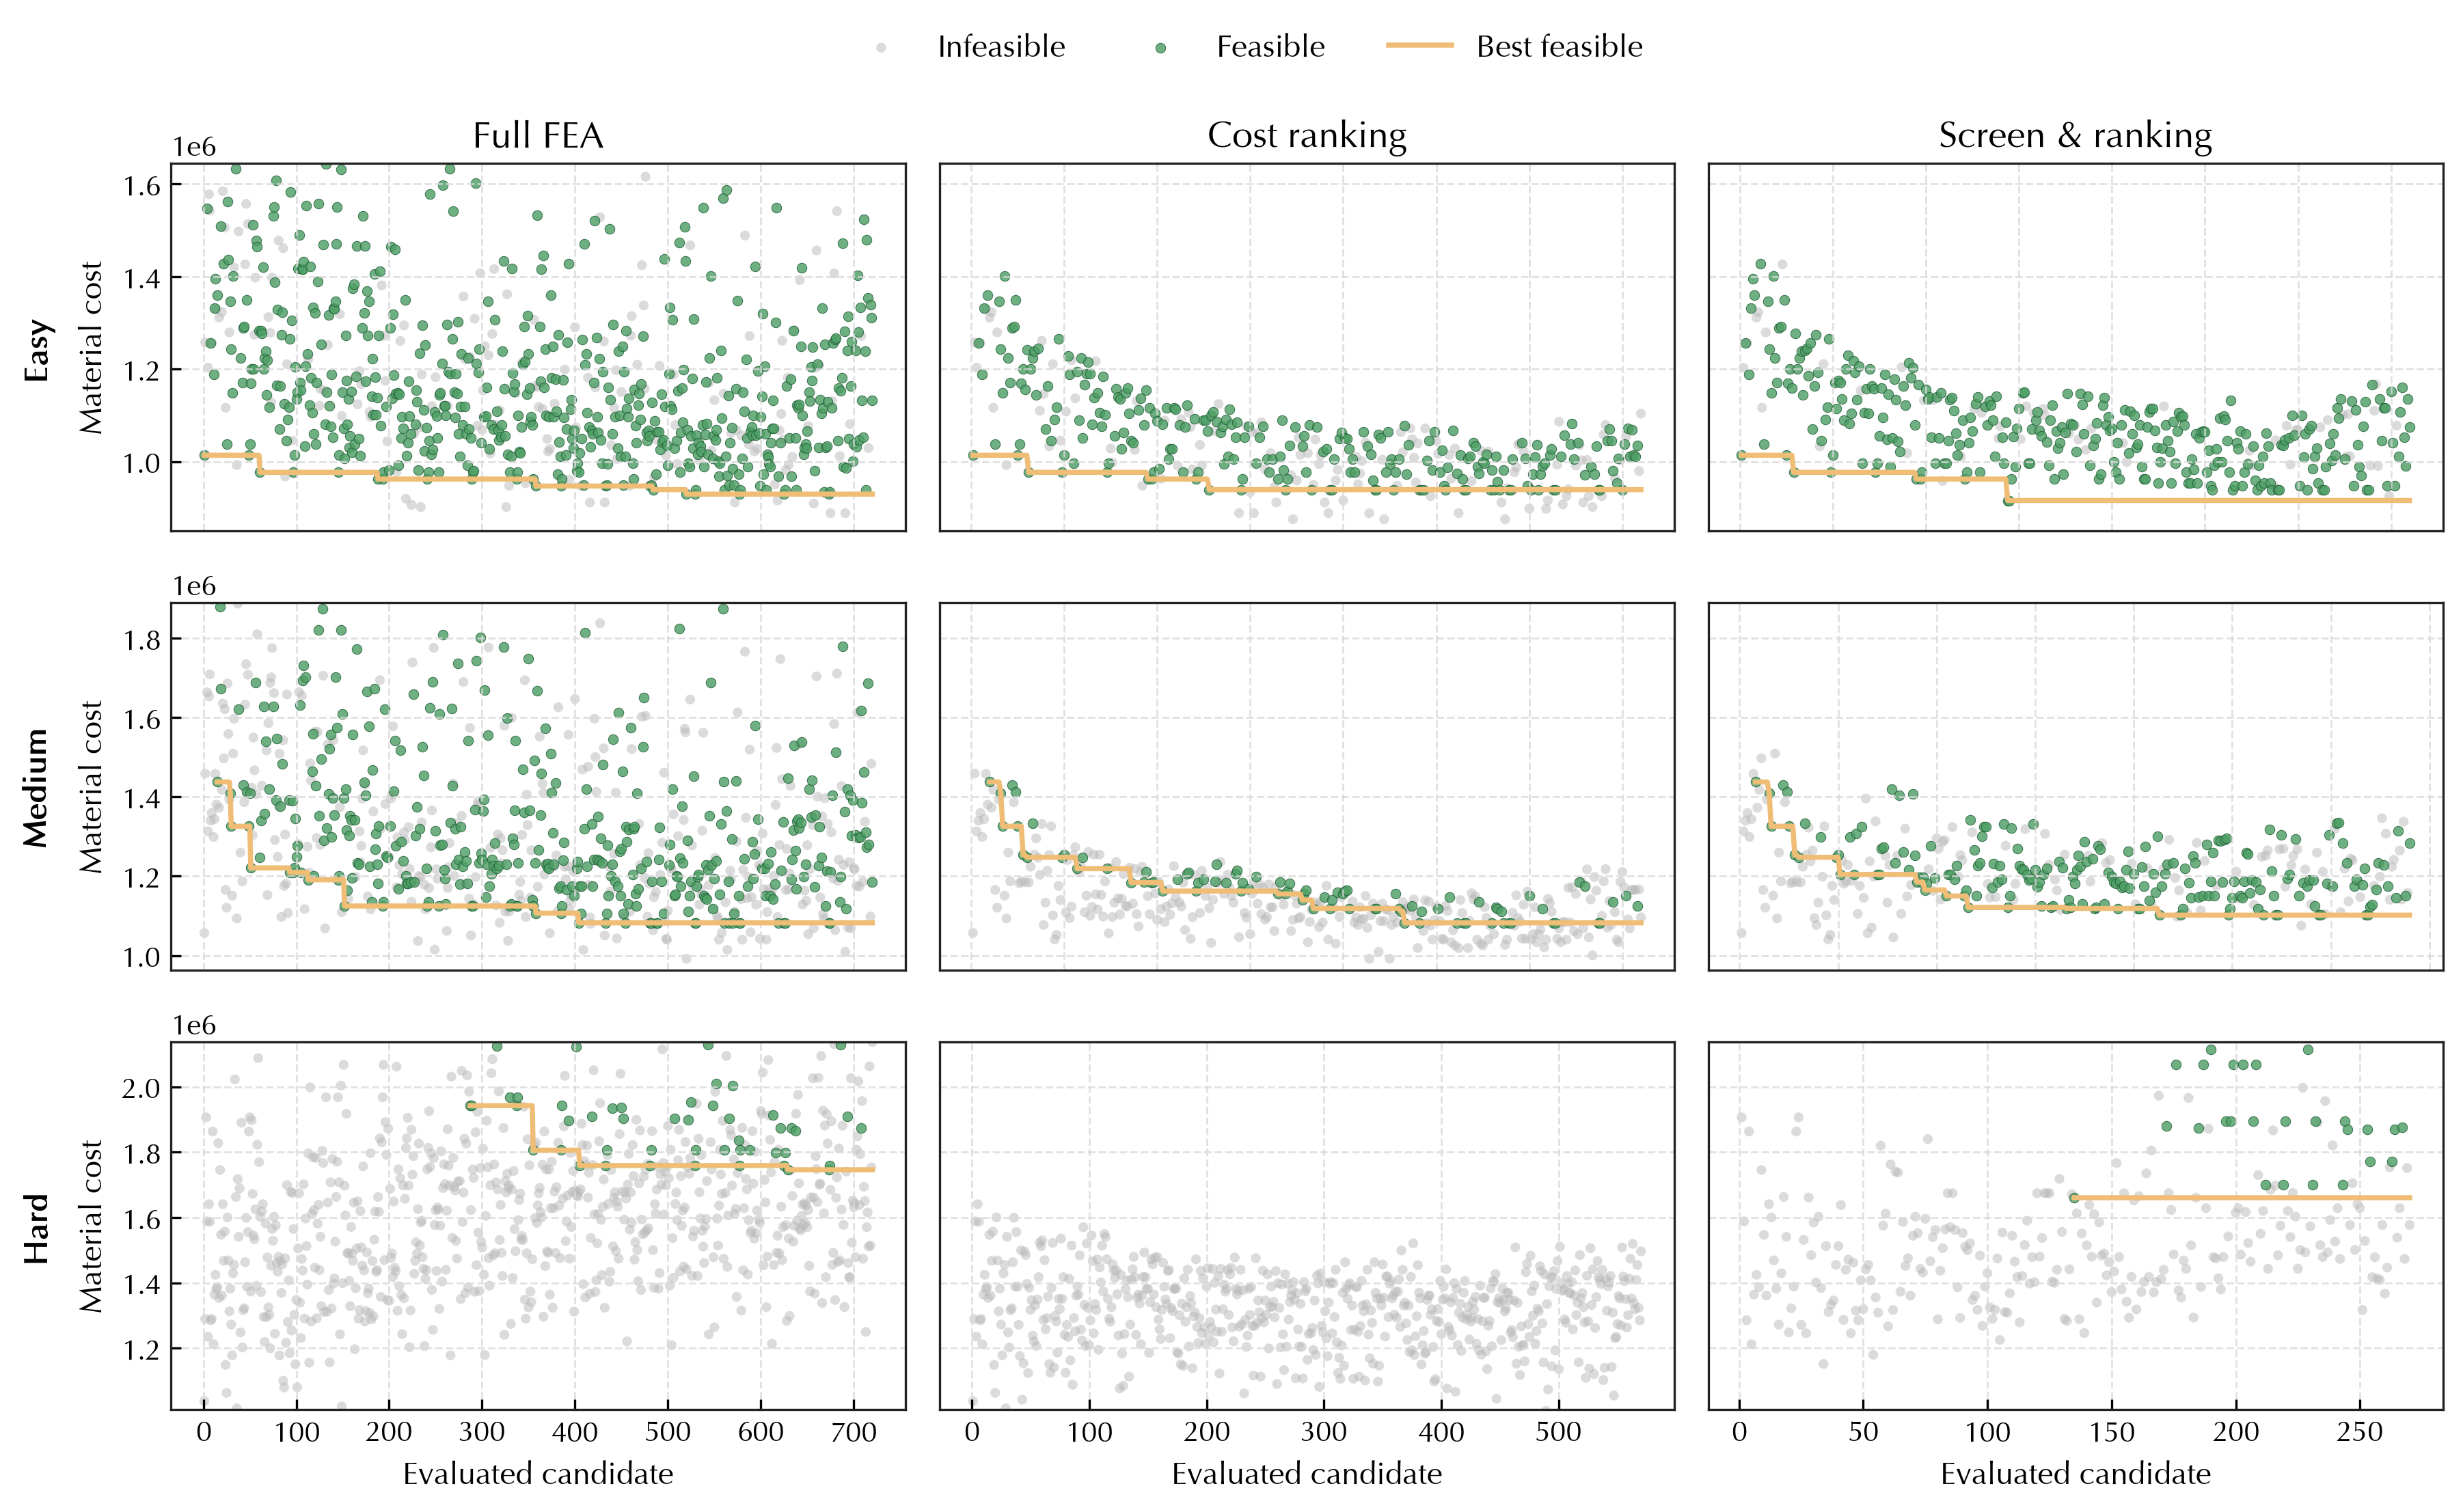
\includegraphics[width=\textwidth]{optimization_case_examples.pdf}
\caption{Representative optimization histories for layouts with different levels of difficulty.}
\label{fig:optimization_case_examples}

\vspace{0.4em}

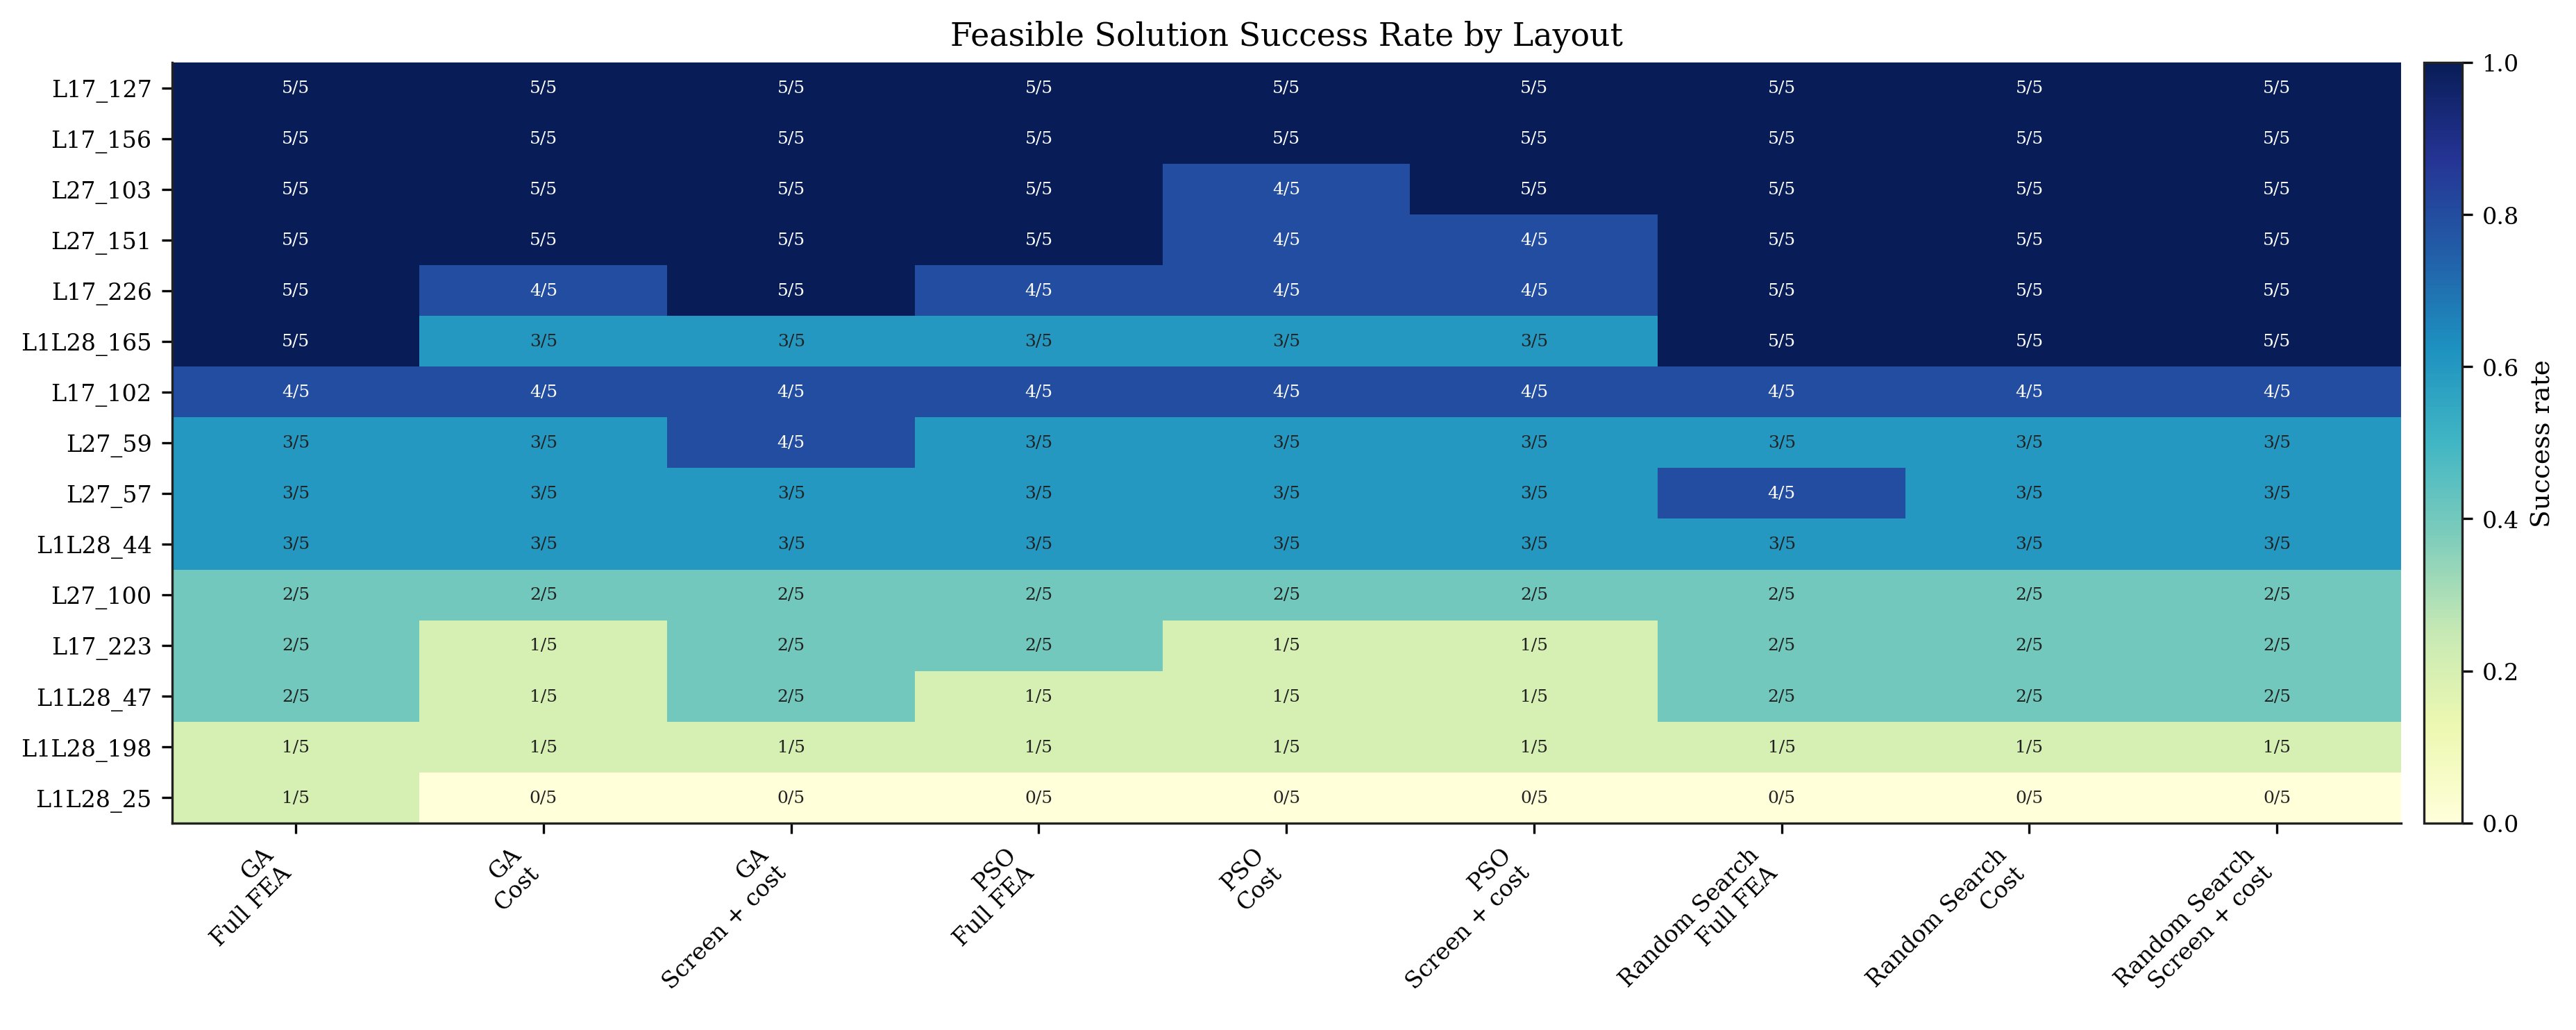
\includegraphics[width=\textwidth]{layout_difficulty_heatmap.pdf}
\caption{Feasible-solution discovery patterns across test layouts and optimization strategies.}
\label{fig:layout_difficulty_heatmap}
\end{figure*}



\subsection{Effectiveness of Online Local Calibration}
\label{subsec:local_calibration_results}
Fig.~\ref{fig:local_calibration_effect} compares the layout-wise prediction errors before and after calibration using 100 local samples. The paired comparisons in Fig.~\ref{fig:local_calibration_effect}(a) and Fig.~\ref{fig:local_calibration_effect}(b) show a consistent shift toward lower error values after calibration, corresponding to lower Brier scores for feasibility prediction and lower MAE for reinforcement estimation. The largest improvements are observed on layouts where the uncalibrated global surrogate has larger errors, indicating that local calibration mainly acts as a bias-correction mechanism rather than replacing the global model.

Table~\ref{tab:local_calibration_results} summarizes representative results using 100 local calibration samples. Three settings are compared to distinguish the effects of global surrogate, direct local learning, and the proposed local calibration strategy. Overall, the calibrated surrogate achieves the best performance for both feasibility prediction and reinforcement estimation.

For the feasibility surrogate, the local-only ablation reduces ECE but does not improve the Brier score, and its feasibility recall is only 0.7265. This result suggests that a model trained only on limited current-layout samples lacks sufficient reliability for conservative screening. In contrast, calibrating the global feasibility probability decreases the Brier score from 0.0749 to 0.0437 and it also decreases the expected calibration error from 0.0895 to 0.0333. The reject rate increases from 0.4708 to 0.5481, while feasibility recall only slightly decreases from 0.9990 to 0.9939. This indicates that calibration improves filtering efficiency while retaining most truly feasible candidates.

For the reinforcement surrogate, the local-only ablation already achieves an MAE of 4.82~t, showing that the mapping from design variables to reinforcement demand can be learned reasonably well within a fixed layout using a small number of samples. Nevertheless, residual calibration of the global prediction further improves both accuracy and bias. The MAE decreases from 11.48~t to 2.04~t, the RMSE decreases from 12.30~t to 2.76~t, and the $R^2$ increases from 0.847 to 0.994. These results confirm that the residual calibration model effectively corrects the systematic error of the global reinforcement surrogate for the current layout.

Fig.~\ref{fig:calibration_sample_efficiency} further examines the sample efficiency of local calibration. The calibration benefit appears with a small number of local samples and then gradually saturates. The feasibility-related results in Fig.~\ref{fig:calibration_sample_efficiency}(a) and Fig.~\ref{fig:calibration_sample_efficiency}(b) show improved probability calibration and screening behavior, while the reinforcement-related results in Fig.~\ref{fig:calibration_sample_efficiency}(c) and Fig.~\ref{fig:calibration_sample_efficiency}(d) show that MAE and bias can be corrected with limited local data. This sample efficiency is important for optimization because the local calibration set is accumulated online from candidates that have already been evaluated by FEA.

Overall, the results confirm that lightweight local calibration can adapt the global surrogate to the current layout without retraining the graph model. Detailed selections of the feasibility probability calibrator and steel residual calibrator under different calibration sample sizes are provided in Appendix Tables~\ref{tab:appendix_feasibility_calibrator} and~\ref{tab:appendix_steel_calibrator}, respectively.

\subsection{Optimization Efficiency and Solution Quality}
\label{subsec:optimization_results}

The calibrated surrogate models are further embedded into optimization procedures to evaluate their practical effect on FEA efficiency and solution quality. 

Table~\ref{tab:optimization_summary_results} summarizes the main quantitative results of the optimization experiments. The cost ratio is computed only for paired cases where both the surrogate-informed strategy and the corresponding full-FEA baseline find feasible solutions. The results show that surrogate-informed evaluation substantially reduces true FEA calls across all three optimizers. The cost-ranking strategy reduces FEA calls by about 50\%--57\%, while adding feasibility screening increases the reduction to about 62\%--66\%. This consistent reduction indicates that the efficiency gain mainly comes from surrogate-based candidate allocation rather than from a specific search algorithm.

The feasible solution discovery rate remains close to that of the full-FEA baseline. With the Screen \& ranking strategy, the success rate decreases only slightly for GA and PSO and remains nearly unchanged for random search. Although surrogate-informed methods may miss feasible designs in some cases, the loss in success rate is small compared with the achieved FEA savings.

Fig.~\ref{fig:optimization_benchmark_results} further compares the distributions of optimization performance. The final material cost results in the second row show that the surrogate-informed strategies do not substantially degrade solution quality. For the Screen \& ranking strategy, the average material cost increase relative to the full-FEA baseline is about 0\%--2\% among paired cases where both strategies find feasible solutions. The first-feasible distributions also show that screening generally reduces the number of FEA calls required to find the first feasible solution, indicating that feasibility prediction helps the optimizer avoid obviously infeasible regions in the early search stage.

In Fig.~\ref{fig:cost_tolerance_analysis}, the horizontal axis represents the allowed cost tolerance relative to the baseline optimum, and the vertical axis represents the proportion of cases that simultaneously satisfy three conditions: a feasible solution is found, the number of FEA calls is reduced, and the final cost is within the specified tolerance. As the tolerance increases from 0\% to about 5\%, the qualified-case ratio increases rapidly and then becomes stable. This trend indicates that, for most cases where full-FEA optimization can find feasible solutions, the surrogate-informed strategy can trade a small cost increase for a substantial reduction in FEA calls.

Taken together, the differences among the three optimizers show that the benefit of surrogate-informed evaluation depends on how effectively each search mechanism uses selectively evaluated candidates. GA benefits most from population diversity and batch-wise comparison, whereas PSO is more sensitive to early screening as the swarm may converge before sufficient calibration samples are accumulated. For random search, the surrogate mainly serves as a pre-evaluation filter because previous evaluations do not guide subsequent sampling. Nevertheless, the consistent reduction in FEA calls across all three optimizers demonstrates that the proposed framework is optimizer-independent in principle. Its fundamental contribution is to increase the information value of each expensive evaluation by directing FEA toward candidates that are more likely to be feasible and economical.

\subsection{Mechanism and Practical Implications}
\label{subsec:mechanism_discussion}

To further clarify how the FEA budget is allocated, Fig.~\ref{fig:candidate_flow_analysis} shows the generation-wise distribution of candidates under the three optimization methods. At each generation or batch, all generated candidates are divided into three mutually exclusive groups: candidates rejected by feasibility screening, candidates that pass the screening but are not selected after cost-based ranking, and candidates submitted to true FEA evaluation. The stacked areas indicate that only approximately 1/3 of the candidates are evaluated by FEA, while the remaining candidates are excluded. The green curve further reports the fraction of candidates that are ultimately confirmed as feasible by FEA. Although the relative proportions differ among GA, PSO, and random search, the overall allocation pattern remains stable throughout optimization, demonstrating that the reduction in FEA calls results from the combined effects of feasibility screening and cost-based ranking.

It is worth noting that some candidates submitted to FEA are still infeasible. This is not a failure of the framework, but a consequence of the conservative screening strategy. The feasibility surrogate is designed to avoid rejecting potentially feasible candidates, so it intentionally retains uncertain or boundary candidates for true verification.

Representative optimization histories are then examined to show how the surrogate modules affect the search trajectory under different layout difficulties. Fig.~\ref{fig:optimization_case_examples} presents three layouts with different feasible candidate ratios, where a higher ratio indicates an easier layout and a lower ratio indicates a more difficult one. In the full FEA baseline, all generated candidates are evaluated, including many high-cost candidates and clearly infeasible candidates. When the reinforcement surrogate is used, evaluations become more concentrated in the low-cost region. However, cost-based ranking alone may still select low-cost but infeasible candidates. After feasibility screening is added, fewer infeasible candidates enter FEA, and the evaluated candidates are more concentrated around promising feasible regions. The best feasible costs remain close to those obtained by full FEA optimization in most cases.

The two surrogate tasks therefore play complementary roles. The reinforcement surrogate reduces evaluations of obviously high-cost candidates and guides the search toward economical designs. The feasibility surrogate reduces evaluations of low-cost but clearly infeasible candidates. Online local calibration further adapts both predictions to the current layout, reducing the influence of global surrogate bias on candidate selection.

As shown in the third row of Fig.~\ref{fig:optimization_case_examples}, the difficult case further reveals why feasibility screening is necessary rather than using cost ranking alone. For this layout, feasible designs are not located in the lowest-cost region; instead, the search needs to move toward larger sections and higher material costs to reach the feasible domain. This trend is evident in the full FEA baseline, where evaluated candidates gradually shift to higher-cost regions and feasible solutions eventually appear. In contrast, the cost-surrogate strategy overemphasizes low-cost candidates, which are mostly infeasible for this layout, and therefore fails to provide useful feedback for moving the search toward feasibility. After feasibility screening is introduced, the screen \& cost ranking strategy filters out low-cost but low-feasibility candidates and retains candidates with higher passing potential. As a result, the search direction becomes closer to the full FEA baseline, enabling feasible solutions to be found with fewer true evaluations.

Finally, layout-level difficulty is analyzed to clarify the applicable scope of the proposed framework. Fig.~\ref{fig:layout_difficulty_heatmap} shows that layout difficulty is a key factor in feasible-solution discovery. Layouts that remain difficult even under full FEA optimization are likely limited by the layout itself or by the section-material design space, rather than by surrogate screening. Therefore, the proposed method is most useful when feasible candidates exist but FEA evaluations are expensive and limited. In such cases, calibrated surrogate can reduce unnecessary evaluations with limited impact on final design quality.
